\uuid{FlbG}
\exo7id{7122}
\titre{exo7 7122}
\auteur{megy}
\organisation{exo7}
\datecreate{2017-02-08}
\isIndication{false}
\isCorrection{false}
\chapitre{Géométrie affine euclidienne}
\sousChapitre{Géométrie affine euclidienne du plan}
\module{Géométrie}
\niveau{L2}
\difficulte{}

\contenu{
\texte{
% angles inscrits
Un antiparallélogramme est un quadrilatère croisé dont les cotés opposés sont deux à deux de même longueur. Soit $ABCD$ un antiparallélogramme. Montrer les assertion suivantes.

\begin{center}
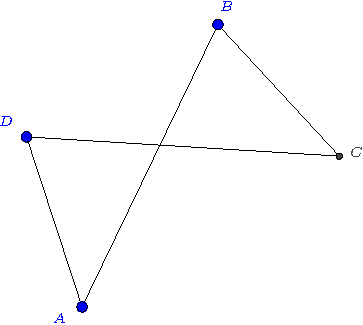
\includegraphics{../images/pdf/FlbG-1.pdf}
\end{center}
}
\begin{enumerate}
    \item \question{Les angles opposés ont la même mesure.}
    \item \question{Les diagonales $(AC)$ et $(BD)$ sont parallèles.}
    \item \question{La médiatrice des diagonales est un axe de symétrie de $ABCD$.}
    \item \question{Deux côtés opposés ont leur point d'intersection situé sur cette médiatrice.}
    \item \question{Le quadrilatère convexe $ADBC$ formé par les deux côtés non croisés et les diagonales est un trapèze isocèle.}
    \item \question{$ABCD$ est inscriptible.}
\end{enumerate}
}
